
\lecture{Hypothesis Test of the Sample Proportion}{hypothesis-test-proportions}
\section{Hypothesis Test of the Sample Proportion}

\title{Hypothesis Test of the Sample Proportion}
\subtitle{Is this the right percentage?}

%\author{Kelly Black}
%\institute{Clarkson University}
\date{7 April 2014}

\begin{frame}
  \titlepage
\end{frame}

\begin{frame}
  \frametitle{Outline}
  \tableofcontents[sectionstyle=show/hide]
\end{frame}


\subsection{Clicker Quiz}


\iftoggle{clicker}{%
  \begin{frame}
    \frametitle{Clicker Quiz}
    
    I call fifty people and ask if they use glasses or another
    corrective lens. Studies indicate that 64\% of people use some
    sort of corrective lens. What is the probability that less than 30
    will say yes?

    \vfill

    \begin{tabular}{l@{\hspace{3em}}l@{\hspace{3em}}l}
      A: 0.28 & B: 0.47  & C: 0.49
    \end{tabular}

    \vfill
    \vfill
    \vfill

  \end{frame}
}



\subsection{Sample Proportion}

\begin{frame}{The Sample Proportion}

  You conduct $n$ trials. Each trial has a probability $p$ for
  ``success'' and a probability of $1-p$ for a different
  result. Define the sample proportion to be 
  \begin{eqnarray*}
    \hat{p} & = & \frac{\mathrm{number~of~successes}}{\mathrm{number~of~trials}}.
  \end{eqnarray*}

  \begin{itemize}
  \item The sample proportion has a mean of $p$, and a standard
    deviation of $\sqrt{\frac{p(1-p)}{n}}$.
  \item Check to see if $p\cdot n \geq 5$, $(1-p)\cdot n \geq 5$ and
    $n\geq 20$. If \textit{all} of these things are true
    \begin{itemize}
    \item $\hat{p}$ is approximately normally distributed
    \item The mean of $\hat{p}$ is mean $p$.
    \item The standard deviation of $\hat{p}$ is
      $\sqrt{\frac{p(1-p)}{n}}$
    \item A $z$-statistic can be approximated using
      \begin{eqnarray*}
        z & = & \frac{\hat{p}-p}{\sqrt{\frac{p(1-p)}{n}}}.
      \end{eqnarray*}
    \end{itemize}

  \end{itemize}



  
\end{frame}



\subsection{Hypothesis Testing}

\begin{frame}
  \frametitle{Left Sided Test of the Proportion}

  You think that the proportion is lower.

  \begin{columns}
    \column{0.25\textwidth}
    \begin{eqnarray*}
      \begin{array}{lrcl}
        H_0: & p & = & \# \\
        H_a: & p & < & \#
      \end{array}
    \end{eqnarray*}

    \column{0.75\textwidth}

    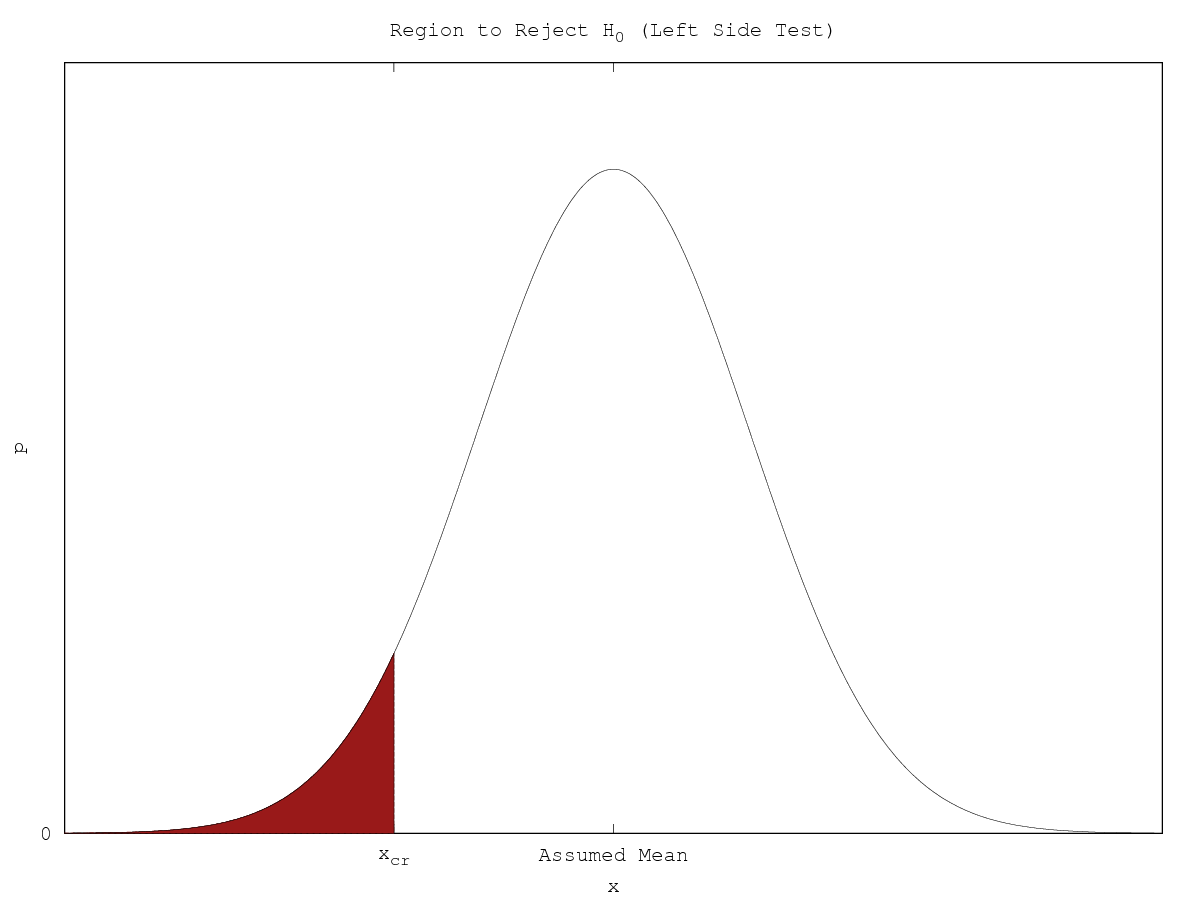
\includegraphics[width=5cm]{img/leftSideHypothesisTest}

  \end{columns}

  \begin{description}
    \only<1>{
    \item[$p$-value Approach] The probability that you do worse than
      $\hat{p}^*$ is the area to the left under the curve. If the area is
      smaller than the significance level ($\alpha$) then it is an
      \textit{unlikely result}.
    }
    \only<2>{
    \item[Classical Approach] The area to the left of $p_{cr}$ is
      equal to the significance level ($\alpha$). If your $\hat{p}^*$ is
      less than this critical value then it is an \textit{unlikely
        result}.
    }
  \end{description}


\end{frame}

\begin{frame}
  \frametitle{Right Sided Test of the Proportion}

  You think that the proportion is higher.

  \begin{columns}
    \column{0.25\textwidth}
    \begin{eqnarray*}
      \begin{array}{lrcl}
        H_0: & p & = & \# \\
        H_a: & p & > & \#
      \end{array}
    \end{eqnarray*}

    \column{0.75\textwidth}

    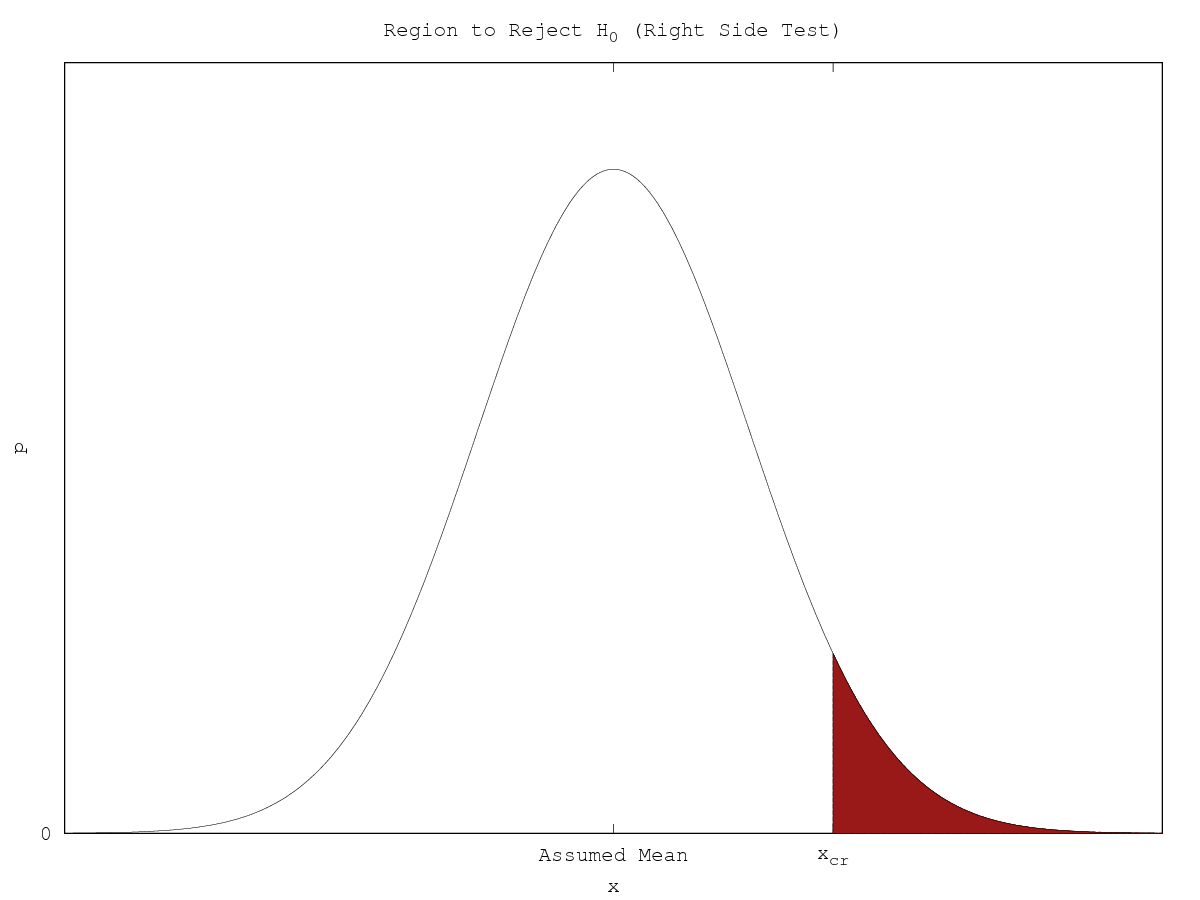
\includegraphics[width=5cm]{img/rightSideHypothesisTest}

  \end{columns}

  \begin{description}
    \only<1>{
    \item[$p$-value Approach] The probability that you do worse than
      $\hat{p}^*$ is the area to the right under the curve. If the area is
      smaller than the significance level ($\alpha$) then it is an
      \textit{unlikely result}.
    }
    \only<2>{
    \item[Classical Approach] The area to the right of $p_{cr}$ is
      equal to the significance level ($\alpha$). If your $\hat{p}^*$ is
      more than this critical value then it is an \textit{unlikely
        result}.
    }
  \end{description}


\end{frame}


\begin{frame}
  \frametitle{Two Sided Test of the Proportion}

  \vspace*{-1em}

  You think that the proportion is different.

  \begin{columns}
    \column{0.25\textwidth}
    \begin{eqnarray*}
      \begin{array}{lrcl}
        H_0: & p & = & \# \\
        H_a: & p & \neq & \#
      \end{array}
    \end{eqnarray*}

    \column{0.75\textwidth}

    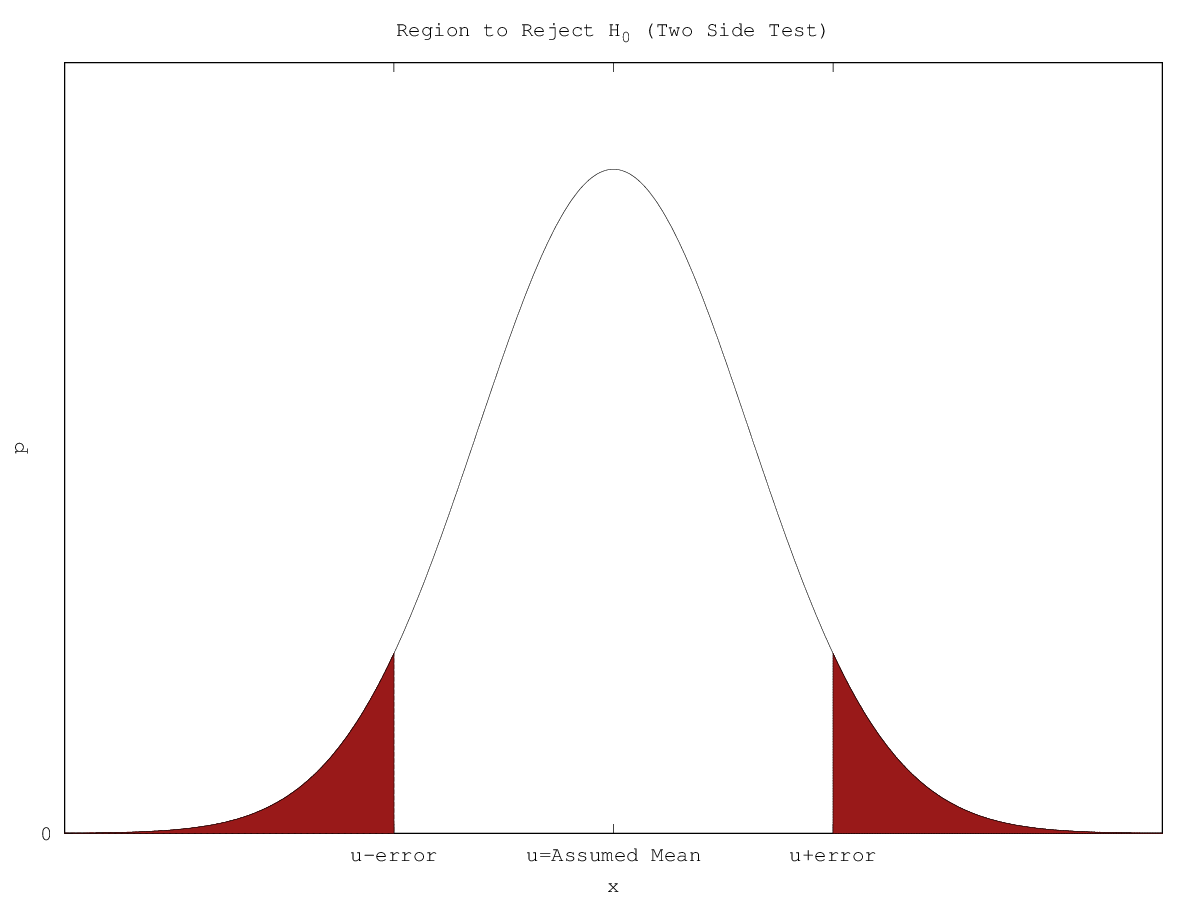
\includegraphics[width=5cm]{img/twoSideHypothesisTest}

  \end{columns}

  \begin{description}
    \only<1>{
    \item[$p$-value Approach] The probability that you do worse than
      $\hat{p}^*$ is the area to the left \textit{plus} the area to the
      right under the curve. If the area is smaller than the
      significance level ($\alpha$) then it is an \textit{unlikely
        result}.  
    } 
    \only<2>{
    \item[Classical Approach] The area to the left of
      $p-\mathrm{error}$ plus the area to the right of
      $p+\mathrm{error}$ is equal to the significance level
      ($\alpha$). If your $\hat{p}^*$ is less than $p-\mathrm{error}$ or
      more than $p+\mathrm{error}$ then it is an \textit{unlikely
        result}.  }
  \end{description}


\end{frame}





\subsection{Examples}

\begin{frame}
  \frametitle{Example: Education Levels}

  \vspace*{-2em}
  You plan on building a new manufacturing plant in a given area. The
  local chamber of commerce says that 80\% of the residents have an
  education level that is at the high-school or better level. You
  believe that the chamber of commerce's figures are too high.

  You call forty people at random and ask them their highest
  educational grade level that they have passed. Twenty-eight say that
  their highest grade level is high-school or better. Are your
  suspicions correct? (Use a 95\% confidence level.)

  \vfill

  \only<2>%
  {
    \begin{eqnarray*}
      \begin{array}{lrcl}
        H_0: & p & = & 0.80 \\
        H_a: & p & < & 0.80
      \end{array}
    \end{eqnarray*}
  }

  \only<3>%
  {
    \begin{eqnarray*}
      & & 
      \begin{array}{rcl@{\hspace{3em}}rcl}
          40*.8 & = & 32, & 40*.2 & = & 8, \\
          N & = & 40, & \hat{p}^* & = & \frac{28}{40},
        \end{array} \\
      z & = & \frac{\frac{28}{40}-.8}{.8(.2)/\sqrt{40}}, ~~ \approx ~~ -1.58
    \end{eqnarray*}
  }
  

  \only<4>%
  {
    The critical $z$-score ($z^*$) is -1.65.
  }

  \only<5->
  {

    {\color{red}
      There is insufficient evidence to reject $H_0$ at the 95\%
      confidence level assuming a normal approximation to the
      proportion with 40 samples.
    }

  }

  \vfill
  
\end{frame}


\begin{frame}
  \frametitle{Example: }

  \vspace*{-2em}
  A recent study indicates that 52\% of people will have to continue
  to work after they retire to supplement their income. You think that
  this number is not high enough. 

  You call five-hundred people at random and ask them if they think
  they will have to continue to work after retirement. Two-hundred and
  eighty-one say that they will have to continue to work. Are your
  suspicions correct?  (Use a 95\% confidence level.)

  \vfill

  \only<2>%
  {
    \begin{eqnarray*}
      \begin{array}{lrcl}
        H_0: & p & = & 0.52 \\
        H_a: & p & > & 0.52
      \end{array}
    \end{eqnarray*}
  }

  \only<3>%
  {
    \begin{eqnarray*}
      500*.52     & = & 260, \\
      500*(1-.52) & = & 240, \\
      N & = & 500, \\
      \hat{p}^* & = & \frac{281}{500}, \\
      z & = & \frac{\frac{281}{500}-.52}{.52(.48)/\sqrt{500}}, \\
      & \approx & 1.88
    \end{eqnarray*}
  }
  

  \only<4>%
  {
    The critical $z$-score ($z^*$) is 1.65.
  }

  \only<5->
  {

    {\color{red}
      There is sufficient evidence to reject $H_0$ at the 95\%
      confidence level assuming a normal approximation to the
      proportion with 500 samples.
    }

  }

  \vfill
  
\end{frame}


\begin{frame}
  \frametitle{Example: }

  \vspace*{-2em}
  A recent study indicates that 15\% of people approve of the job that
  the congress is doing. You think that this is not right. 

  You call four-hundred people at random and ask them if they approve
  of the job that the congress is doing. Fifty people say that they
  approve of the work that the congress is doing. Are your suspicions
  correct?  (Use a 95\% confidence level.)

  \vfill

  \only<2>%
  {
    \begin{eqnarray*}
      \begin{array}{lrcl}
        H_0: & p & = & 0.15 \\
        H_a: & p & \neq & 0.15
      \end{array}
    \end{eqnarray*}
  }

  \only<3>%
  {
    \begin{eqnarray*}
      400*.15     & = & 60, \\
      400*(1-.15) & = & 340, \\
      N & = & 400, \\
      \hat{p}^* & = & \frac{50}{400}, \\
      z & = & \frac{\frac{50}{400}-.15}{.15(.85)/\sqrt{400}}, \\
      & \approx & -1.400
    \end{eqnarray*}
  }
  

  \only<4>%
  {
    The critical $z$-score ($z^*$) is $\pm 1.96$.
  }

  \only<5->
  {

    {\color{red} 

      There is not sufficient evidence to reject $H_0$ at the 95\%
      confidence level assuming a normal approximation to the
      proportion with 500 samples.  

    }

  }

  \vfill
  
\end{frame}




%%% Local Variables: 
%%% mode: latex
%%% TeX-master: "IntroStats"
%%% End: 

% LocalWords:  pausesection hideothersections sectionstyle
